
\chapter{Project schedule from Initial Document}
\label{app:project_schedule}

    You can see the project schedule we included in the Initial document in \ref{app:project_schedule} on page \pageref{app:project_schedule}. We have distinguished categories of tasks in the schedule through colour coding. Green represents tasks that are directly related to the completion of the project, whether it be research, design, implementation, or testing. Blue bars represent tasks related to the deliverables required by the university besides the Android Image. Grey tasks are periods of time reserved to focus on other courseworks or on exams. Finally, orange tasks are for the completion of secondary project objectives.
    
    \begin{landscape}
    \begin{figure}[H]
    	% [H] means put the figure HERE, directly when you input this code.
    	\centering
    	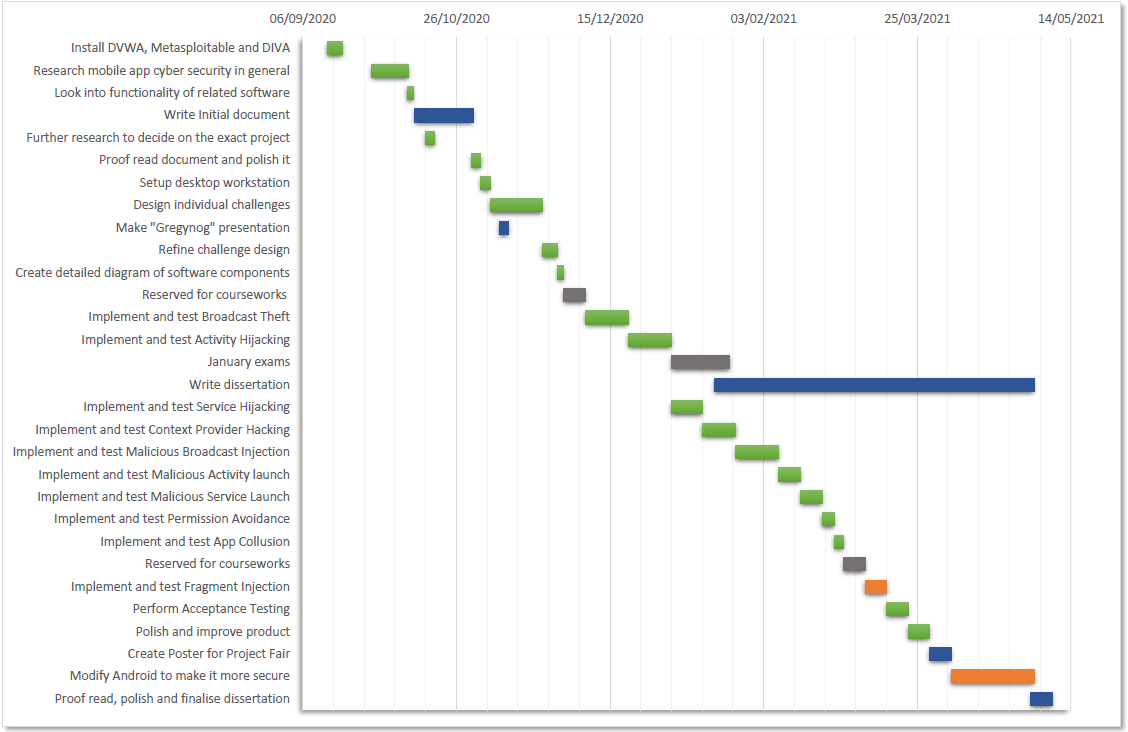
\includegraphics[width=1\linewidth]{./graphics/schedule.PNG}
    	
    	% Caption is defined with a short and long version. The short 
    	% version is shown in the List of Figures section, and the long 
    	% version is used directly with the figure. 		
    	\caption[Project schedule.]{The Project Schedule we had in the Initial Document for this project.}
    	
    	% For figures, \label should be defined after the caption to ensure 
    	% proper figure numbering.
    	\label{fig:schedule}
    \end{figure}
    \end{landscape}

\chapter{Supplementary Data}
\label{app:supplementary_data}

The results of large ablative studies can often take up a lot of space, even with neat visualization and formatting. Consider putting full results in an appendix chapter and showing excerpts of interesting results in your chapters with detailed analysis. You can use labels and references to refer the reader here for the full data.
